\chapter{Desenvolvimento do Software}
\thispagestyle{empty} % retira numeracao da pagina, conforme as normas de apresentacao.


Neste capítulo será discutido a aplicação de algumas das práticas e metodologias de desenvolvimento de software que se demonstraram adequadas ao contexto e escopo do projeto e foram utilizadas no desenvolvimento da aplicação. Também serão apresentados seus conceitos mais importantes e de que maneira se relacionam com o nosso projeto de forma a motivar a sua aplicação.

O desenvolvimento tradicional, também conhecido como Desenvolvimento em Cascata, acontece de forma linear e em várias fases, onde cada uma utiliza o resultado da fase anterior. Ou seja, primeiro a equipe realiza a análise, seguida do design, implementação, teste e assim por diante. Em contrapartida, o Desenvolvimento Ágil é baseado na idéia de desenvolvimento incremental e iterativo, em que as fases que compõem o Ciclo de Vida de Desenvolvimento de Sistemas (CVDS) são revisitadas repetidamente. O \textit{software} é melhorado iterativamente usando o \textit{feedback} do cliente para convergir em soluções \cite{book:szalvay}. 

No contexto do nosso projeto, o caráter incremental e evolutivo das Metodologias Ágeis permitiu que o planejamento do desenvolvimento subsequente fosse feito a cada reunião com o orientador do projeto, bem como a avaliação das tarefas que foram planejadas na reunião anterior, tendo assim um ritmo bem definido que ocorria de forma iterativa, onde todas as fases necessárias puderam se repetir a cada ciclo. Ao final de cada uma destas iterações, foi entregue uma versão utilizável do \textit{software}, começando por uma versão bem simples na primeira iteração até que foi alcançado o resultado desejado ao final do desenvolvimento.

Para as disciplinas de Projeto I e II, foi necessário adotar uma metodologia que atendesse a necessidade do desenvolvimento orientado, do \textit{feedback} contínuo e da possibilidade de mudanças ao longo do curso da execução sem maiores impactos. Desta forma, no sentido mais amplo da execução do projeto, foram adotadas algumas Metodologias Ágeis de Desenvolvimento de Software, dado as suas características fundamentais:

\begin{enumerate}
    \item O envolvimento do cliente desde cedo
    \item O desenvolvimento iterativo
    \item Equipes auto-organizadas
    \item Adaptação à mudanças
\end{enumerate}

Além das características supracitadas, que se referem ao processo macro do desenvolvimento, foi identificado, de maneira mais pontual, a necessidade de adotar a programação em par, dado que o projeto foi desenvolvido em dupla e ambos os autores deveriam compreender todos os detalhes de implementação e pudessem auxiliar um ao outro em face dos possíveis obstáculos encontrados, além de revisar crítica e continuamente o trabalho do outro para que a qualidade almejada fosse mantida, reduzindo a possibilidade de introdução de \textit{bugs} e a tomada de decisões de \textit{design} inadequadas para a solução. Também no que se refere a qualidade de \textit{Software}, o desenvolvimento orientado a testes, as refatorações, medições e a integração continua foram meios de manter a qualidade das entregas e a garantia de funcionamento integral do produto a medida que novas funcionalidades eram adicionadas.

\section{Metodologia}

Dentre as metodologias ágeis existentes na atualidade, o SCRUM e o \textit{Extreme Programming} foram escolhidos como metodologia de desenvolvimento para este projeto, dado as necessidades identificadas acima.

O Scrum e o \textit{Extreme Programming} são os membros da família de metodologias ágeis de desenvolvimento de \textit{software} que têm atraído significativa atenção entre os profissionais de \textit{software} durante os últimos anos, ambos tem sido largamente aceitos como duas das mais importantes abordagens ágeis \cite{book:xp}.
O método \textit{Extreme Programming} tem seus conceitos bem definidos acerca da atividade de programação, como na programação em par, padrões de codificação, desenvolvimento orientado à testes, refatoração e integração contínua. Já o Scrum se concentra na gestão de projetos de software. Por essa divisão clara das aplicabilidades de ambas metodologias, foi possível adotá-las de forma complementar para o desenvolvimento deste projeto.

\subsection{Aplicação do SCRUM}

O Scrum parte da premissa de que o desenvolvimento de software é complexo e imprevisível demais para ser planejado antecipadamente com exatidão. Em vez disso, o controle de processos empíricos deve ser aplicado para assegurar a visibilidade, inspeção e adaptação.
As diferentes variáveis ambientais e técnicas (tais como período de tempo, qualidade, requisitos, recursos, tecnologias de implementação e ferramentas, e até mesmo métodos de desenvolvimento) devem ser controladas constantemente a fim de poder se adaptar às alterações de forma flexível. Isto é obtido através de um processo de desenvolvimento iterativo e incremental.

\begin{figure}[H]
    \centering
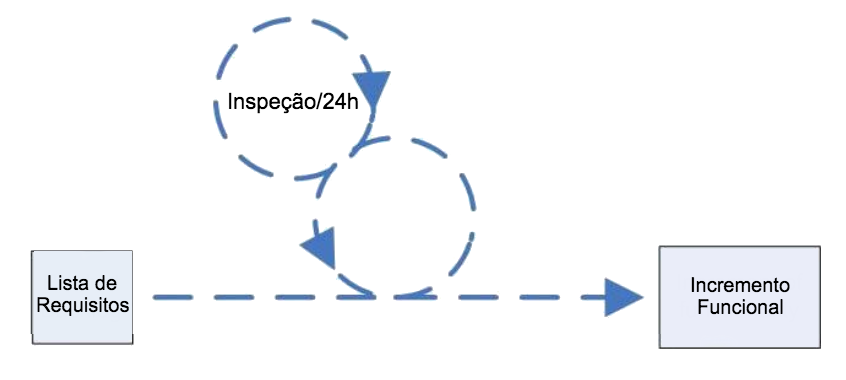
\includegraphics[scale=0.45]{3_1}
    \caption{Esqueleto SCRUM}
    \label{scrumesqueleto}
\end{figure}

O esqueleto de scrum é mostrado na Figura \ref{scrumesqueleto} \cite{book:schwaber}

O círculo inferior representa uma iteração das atividades de desenvolvimento que ocorrem sequencialmente. O resultado de cada iteração é um incremento do produto. O círculo superior representa a inspeção diária que ocorre durante a iteração, em que os membros da equipe se reúnem para inspecionar as atividades uns dos outros e fazer as adaptações necessárias. Uma lista de requisitos é o que conduz a iteração. Este ciclo se repete até que o projeto seja concluído.

O Scrum implementa este ciclo iterativo e incremental através de três papéis: o \textit{Product Owner}, a equipe, e o \textit{Scrum Master}.


\begin{itemize}
    \item O \textit{Product Owner} é responsável por representar os interesses de todos os interessados no projeto do sistema final. Ele mantém o \textit{Product Backlog}, isto é, uma lista priorizada de requisitos do projeto com tempos estimados para transformá-los em funcionalidade do produto concluído.
    \item A Equipe é responsável pelo desenvolvimento das funcionalidades. As equipes são auto-geridas, auto-organizadas, interfuncionais, e eles são responsáveis por descobrir como transformar o \textit{Backlog} do Produto em um incremento de funcionalidade dentro de uma iteração e gerir o seu próprio trabalho para fazê-lo. Os membros da equipe são coletivamente responsáveis pelo o sucesso de cada iteração e do projeto como um todo.
    \item O \textit{Scrum Master} preenche a posição normalmente ocupada pelo gerente de projeto, mas seu papel é ligeiramente diferente. Enquanto o gerente de projeto tradicional é responsável pela definição e gestão do trabalho, o \textit{Scrum Master} é responsável por gerenciar o processo Scrum, ensinando o Scrum para todos os envolvidos no projeto, implementando o Scrum que caiba dentro da cultura da organização em questão, entregando os benefícios esperados, e assegurando que todos sigam as regras e práticas do Scrum.
\end{itemize}

No desenvolvimento deste projeto, foram atribuídos os papéis de \textit{Product Owner} para o professor orientador do projeto, e os autores dividiam as atribuições de \textit{Scrum Master} e da equipe. 

\begin{figure}[H]
    \centering
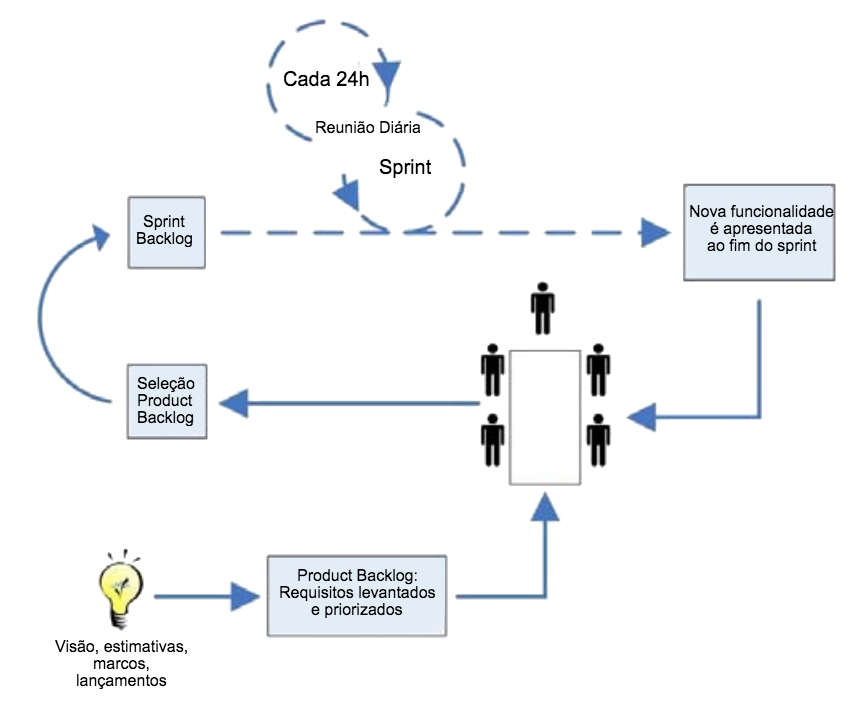
\includegraphics[scale=0.45]{3_2}
    \caption{Esqueleto SCRUM detalhado}
    \label{figura2}
\end{figure}

O fluxo Scrum detalhado é mostrado na Figura \ref{figura2} \cite{book:schwaber}.

O projeto de um Scrum começa com o vislumbre do sistema a ser desenvolvido. Em seguida o \textit{Product Backlog} é criado, uma lista contendo todos os requisitos já conhecidos. O \textit{Product Backlog} é priorizado e dividido em lançamentos propostos. 

No contexto deste projeto, o vislumbre, ou visão do projeto, foi feito na apresentação da proposta ao professor orientador, que por sua vez adicionou e reviu o seu escopo junto aos autores. Neste momento, tanto os autores quanto o professor orientador, exerceram o papel de \textit{Product Owner}, por serem todos partes interessadas no produto. O \textit{Product Backlog}, foi definido na disciplina de Projeto Final I, cujo resultado se deu na forma do documento de Especificação de Requisitos do Software, detalhada no Capítulo 4.

No Scrum, dodo o trabalho é feito em divisões temporais chamadas de \textit{Sprints}. Cada \textit{Sprint} é uma iteração 30 dias consecutivos ou outro intervalo que melhor se adeque a organização.

Cada \textit{Sprint} é iniciado com uma reunião de planejamento, onde o \textit{Product Owner} e a equipe se juntam para planejar o que será feito para o próxima iteração. O \textit{Product Owner} diz à equipe o que é desejado e para quais requisitos tem o nível de prioridade mais alto no \textit{Product Backlog}, a equipe diz ao \textit{Product Owner} o quanto daquilo acredita que pode se transformar em funcionalidade ao longo do próximo \textit{Sprint}.
Depois de decidir o que deve ser feito, a equipe desenvolve o \textit{Sprint Backlog}, isto é, uma lista de tarefas que devem ser executadas para entregar um incremento completo de funcionalidade do produto potencialmente utilizável até o final da iteração. As tarefas na lista emergem a medida que o \textit{Sprint} evolui e devem ser divididas de modo que cada uma leve entre 4 e 16 horas para ser concluída.
A cada dia, a equipe se reúne para uma reunião de 15 minutos chamada Reunião Diária. No Scrum diário, cada membro da equipe responde a três perguntas: O que você fez neste projeto desde a última reunião diária? O que você vai fazer antes da próxima reunião? Você tem obstáculos? O objetivo da reunião é sincronizar o trabalho de todos os membros da equipe e para agendar quaisquer reuniões que a equipe precise para transmitir o seu progresso.

Para este projeto, os \textit{Sprints} tiveram duração semanal e eram delimitados pelas reuniões de orientação, onde era feita a revisão das entregas, o \textit{Sprint Review} e o planejamento subsequente,  o \textit{Sprint Planning}, com os próximos requisitos selecionados e priorizados pelo professor orientador no papel do \textit{Product Owner} e acordados com os autores, na função de \textit{Scrum Masters} e Equipe, formando o \textit{Sprint Backlog}. O Scrum diário era realizado pelos autores durante as sessões de desenvolvimento, onde se discutia as decisões de implementação, os obstáculos encontrados e avaliava-se as atividades do dia.

\subsection{Práticas de \textit{Extreme Programming}}


Além de princípios do Scrum, utilizamos de atividades propostas pelo  \textit{Extreme Programming}, ou XP. De acordo com Teles \cite{book:xp}, o XP é um processo de desenvolvimento de \textit{software} voltado para:

\begin{itemize}
    \item Projetos cujos requisitos são vagos e mudam com frequência.
    \item Desenvolvimento de sistemas orientados a objeto.
    \item Equipes pequenas, preferencialmente até 12 desenvolvedores.
    \item Desenvolvimento incremental (ou iterativo), onde o sistema começa a ser implementado logo no início do projeto e vai ganhando novas funcionalidades ao longo do tempo.
\end{itemize}

Baseado nisso o XP se tornou um processo determinante para o bom andamento do desenvolvimento do \textit{software}. Entretanto, devido ao ambiente em que o desenvolvimento estava inserido, por exemplo não existia um cliente, papel que a maioria das vezes foi representado pelo orientador, foram adotadas apenas algumas da práticas do XP.

Algumas dessas práticas foram, o jogo do planejamento, onde a equipe se reunia semanalmente para obter \textit{feedbacks} e baseado nisso realizar o planejamento da semana, sempre priorizando as tarefas julgadas mais importantes para o sistema. Programação em par, embora não executada o tempo todo, como prega o XP, esta prática foi utilizada diversas vezes pela equipe quando foi necessário o desenvolvimento de de partes mais complexas do sistema. Dessa forma os dois desenvolvedores contribuíam diretamente com revisões e opiniões enquanto a funcionalidade era construída, gerando uma solução mais eficaz ao final. Código Coletivo, todos os desenvolvedores eram responsáveis e possuíam acesso a todo o código. Código padronizado e \textit{design} simples. Além disso a Integração Contínua, na qual as novas funcionalidades do sistema eram incorporadas ao código o mais rápido possível. Integração coberta por testes automatizados que garantem que o sistema ainda esteja funcionando após cada integração. Tais testes foram criados utilizando a prática conhecida como TDD descrita abaixo.

\subsection{Testes do Software}

O \textit{Test Driven Development} (TDD) \cite{book:beck}, é uma técnica de desenvolvimento de software que combina as técnicas \textit{test-first development} (TFD), no qual você escreve seus testes antes do código, e refatoração. Ambas muito relacionadas com o desenvolvimento ágil. Segundo Beck (2003), criador do TDD, além de um dos idealizadores do Manifesto Ágil, Desenvolvimento Orientado a Testes deve encorajar \textit{design} simples e inspirar confiança. É uma prática de programação e não apenas técnicas para teste, apesar de gerar um conjunto de testes ao final, nem sempre tais testes por si só são satisfatórios para o projeto como um todo.

O ciclo do TDD é definido como um simples sequência de tarefas a ser executadas e repetidas até que o resultado obtido seja satisfatório. Apesar de existirem variações, a forma mais comum de se realizar isso é através do uso de testes unitários automatizados.

O primeiro passo é escrever o teste. A cada nova funcionalidade os testes devem ser escritos primeiro, antes de qualquer linha de código da mesma. Este teste deve falhar, caso isto não aconteça tal funcionalidade pode já estar implementada ou o teste está errado. O \textit{test-first development} permite que o programador, neste momento, esteja completamente focado nos requisitos para se implementar essa funcionalidade, não sendo influenciado por como ele pretende implementa-la, eliminando o risco de testes que só funcionam para determinados códigos.

O segundo passo é rodar todos os testes para verificar se o novo falha. O objetivo é validar se o teste que acabou de ser escrito não passa sem que o código requerido esteja implementado, o que o caracterizaria com um teste inútil, aumentando a confiança de que este esteja testando corretamente.
O terceiro passo é escrever o código que faça o novo teste passar. Nesta etapa não é necessário que o código esteja perfeito, e sim o mais simples possível. O objetivo é garantir uma versão inicial que atenda aos requisitos, mesmo que de forma pouco eficiente. Eficiência, ou qualquer outro problema que este venha a ter, serão tratados nos próximos passos.
O quarto passo é novamente rodar o testes. Desta vez é esperado que eles todos passem, garantindo assim que eles realmente cumprem o objetivo.

O quinto passo é a refatoração. Nesta etapa o código precisa ser melhorado o quanto for necessário. Como nesta etapa podem surgir diversas modificações os testes escritos anteriormente se fazem fundamentais, e devem ser executados a todo tempo para auxiliar a refatoração. Testes passando indicam que suas modificações não mudaram o comportamento do código.

Os cinco passos então são repetidos para cada novo teste necessário a funcionalidade. O tamanho dos passos devem sempre ser pequenos, e os testes devem ser executados continuamente.

Os testes gerados por tal prática são muito importantes para este projeto para que possamos garantir que novas integrações não introduzam problemas ao código já existentes, principalmente porque este é aberto para contribuições da comunidade. 

Primeira e talvez a principal vantagem que a prática trouxe ao desenvolvimento do Integra UFF foi o aumento da qualidade do código, e consequentemente do produto. Com o constante suporte dos testes, o Desenvolvimento Orientado a Teste ofereceu uma grande validação dos requisitos, pois demanda foco nas especificações do produto para que seja possível escrever os testes primeiro. Além de facilitar a depuração de erros no futuro, já que a prática encoraja testes simples, permitindo a detecção de erros mais facilmente. O encorajamento em produção de testes simples, geralmente levam a produção de códigos simples e mais claros. No futuro do projeto, códigos mais legíveis e bem construídos contribuirão para manutenção, mudanças e desenvolvimento de novas funcionalidades.

Toda mudança ou nova funcionalidade exige que você execute todos os testes já criados tanto referentes a tal mudança quanto os outros. Isso aumentou a confiabilidade no sistema, já que se eles estiverem passando isso garante que o sistema continua funcionando do modo esperado. Um conjunto de testes bem feito provê localização de defeitos, detecta mudança indesejadas, aumenta a confiança do desenvolvedor, diminui os riscos. Além de permitir rápida reação a mudanças de escopo, o que confirma sua ótima utilidade em processos ágeis.

\section{Gerência de Configuração do \textit{Software}}

"Gerência de Configuração de \textit{Software}, também chamado gerência de mudanças, é um conjunto de atividades elaboradas para gerenciar mudanças por identificação de produtos de trabalho que são suscetíveis a mudanças, estabelecendo relações entre eles, definindo mecanismos para gerenciar diferentes versões destes produtos de trabalho, controlando mudanças impostas, e auditando e relatando a cada mudança feita." (PRESSMAN, 2010)

O \textit{Git} \cite{website:git} foi a ferramenta escolhida para a realizar a gerência de configuração do projeto. Ele é um sistema de controle de versionamento gratuito e possui código aberto. O \textit{Git} possui um avançado sistema de ramos, permitindo a criação, junção e remoção de ramos localmente. Além de ser extremamente rápido comparado a outros sistemas, devido ao fato da maioria de suas ações serem realizadas localmente, evitando diversas comunicações com um servidor remoto. Isto é possível pois ele é distribuído, o que significa que cada usuário possui uma cópia completa e funcional do repositório, podendo até mesmo servir de \textit{backup}.

\begin{figure}[H]
    \centering
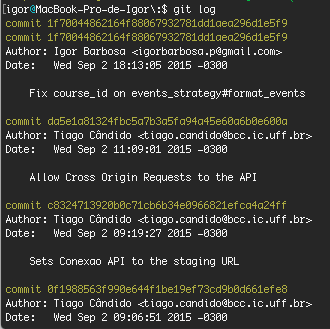
\includegraphics[scale=1]{3_3}
    \caption{Exemplo do histórico de versões do \textit{Git}}
    \label{figura3}
\end{figure}

O repositório \textit{Git} foi compartilhado remotamente na plataforma \textit{Github} \cite{website:github}, um serviço \textit{web} que oferece, além do repositório, uma excelente interface gráfica facilitando assim a visualização do código, novas modificações, histórico, mudanças entre revisões, métricas e etc. E também um robusto sistema de colaboração, permitindo que qualquer pessoa possa visualizar e contribuir com o código hospedado caso este seja aberto, como é o caso deste projeto.

\begin{figure}[H]
    \centering
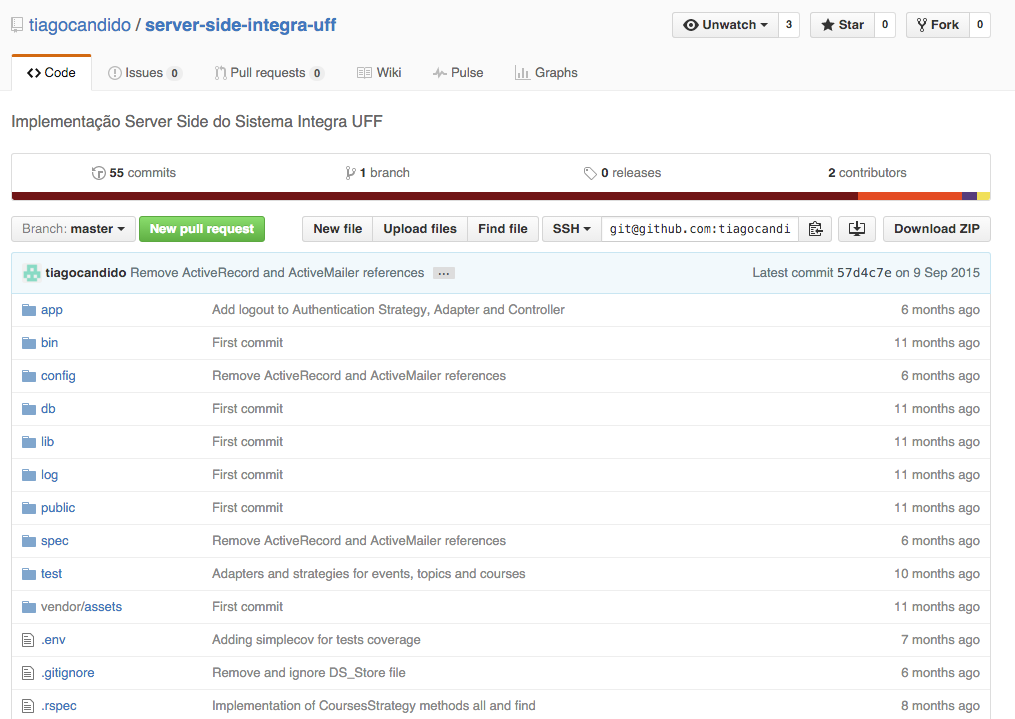
\includegraphics[scale=0.45]{3_4}
    \caption{Interface do \textit{Github}}
    \label{figura4}
\end{figure}



\section{Qualidade de Software}

Garantir a qualidade do código, ou até mesmo definir o termo não é uma tarefa fácil. Existem diversas maneiras de se implementar determinadas soluções e a forma como um desenvolvedor interpreta um código como de qualidade pode diferir muito da opinião de outro desenvolvedor.

Neste projeto foram empregadas várias práticas para que a qualidade do código e do produto final em si fosse mantida ao longo do desenvolvimento. Algumas delas, as quais se inserem no contexto das metodologias ágeis, já foram citadas. Os testes automatizados garantem que os requisitos do sistema sejam atendidos e que continuem funcionando bem a cada nova adição ao código. Ademais foi identificada a necessidade de realizar algumas análises mais quantitativas em cima do código, devido a intenção de receber contribuições ao código aberto. Em vista disto foi decido rodar algumas métricas sobre ele.

\subsection{Linhas de Código}

A quantificação das linhas de código é uma das formas mais simples e antigas para se analisar um determinado \textit{software}. Esta se dá pelo cálculo de todas as linhas não nulas e não comentadas da fonte do código, e exibida de forma geral, arquivo por arquivos, organizadas por módulos, camadas da arquitetura, ou por código de produção versus código de teste.

As linhas de código sozinhas não oferecem muita utilidade para uma análise de qualidade. Porém esta pode ser combinada com os testes automatizados para se obter uma razão entre linhas de código e linhas de teste, que podem indicar o tipo de abordagem utilizada para os testes da aplicação e se os testes são suficientes. E dependendo do tipo de forma que a quantidade de linhas forem exibidas, elas podem ser úteis para perceber módulos do \textit{software} que estão muito grandes e possivelmente acumulando muitas responsabilidades, necessitando de melhorias.

O \textit{framework Ruby on Rails} utilizado para o desenvolvimento deste projeto possui o comando \textit{rake stats} que permite obter tais informações rapidamente como mostrado na figura \ref{figura5}.

\begin{figure}[H]
    \centering
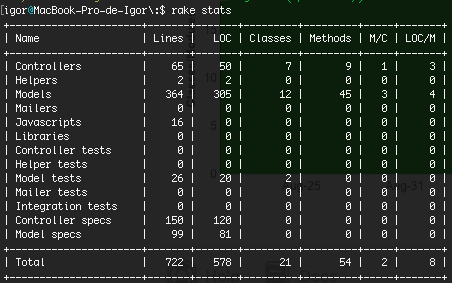
\includegraphics[scale=1]{3_5}
    \caption{Informações de linhas de código do projeto}
    \label{figura5}
\end{figure}

\subsection{Complexidade}

Para obter números acerca da complexidade do código foram utilizadas duas métricas em conjunto:

\begin{itemize}
    \item Complexidade ciclomática - Definida por Thomas McCabe, por isso também chamada de complexidade de McCabe, ela é uma conta que mede a quantidade de caminhos de execução independentes a partir de um código fonte. De acordo com McCabe (1976), ela foi concebida para se adequar a nossa noção intuitiva de complexidade.
    \item Métrica ABC - Esta métrica agrega o número de atribuições, ramos e condições (\textit{assignments, branches} e \textit{conditionals}) de uma unidade do código. Sendo a parte da avaliação dos ramos muito similar a complexidade ciclomática. Ela foi pensada para ser aplicada em diversos tipos de linguagem e estilos, o que permite comparar as pontuações geradas por ela entre diferentes bases de código. Embora seja provavelmente ineficaz em linguagem não imperativas.
\end{itemize}

\subsection{\textit{Churn}}

A métrica \textit{Churn} mensura o número de vezes que um arquivo do seu código fonte mudou ao longo do tempo, calculado pelo número de versões que aquele arquivo possui no histórico do seu controle de versionamento. Como a métrica de linhas de código o número absoluto de \textit{Churn} de um arquivo sozinho não é muito útil. Este se torna valioso quando combinado com a métrica de complexidade como mostrado no gráfico da figura \ref{figura6}, auxiliando a equipe a perceber quais os arquivos causam maiores impactos ao desenvolvimento.

\begin{figure}[H]
    \centering
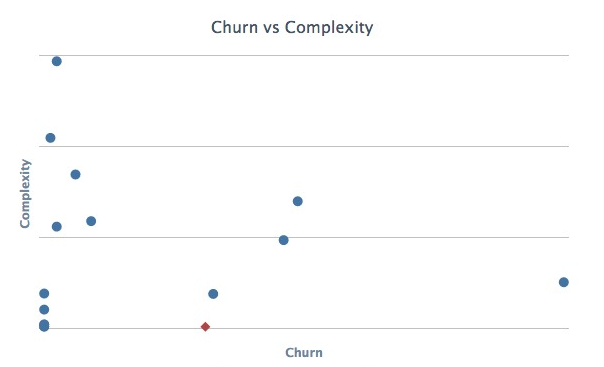
\includegraphics[scale=0.7]{3_6}
    \caption{Gráfico \textit{Churn} vs Complexidade}
    \label{figura6}
\end{figure}

O gráfico apresenta quatro quadrantes que permitem as seguintes análises: 

\begin{enumerate}
    \item Superior direito — Arquivos com alta complexidade e muitas modificações. Arquivos neste quadrante são bons candidatos a serem refatorados, já que a sua manutenção é frequente e a complexidade alta impacta os desenvolvedores negativamente e regularmente. 
    \item Superior esquerdo — Alta complexidade mas não muita mudança. Lidar com arquivos deste quadrante é um pouco mais complexo já que o custo da sua manutenção é alto devido a sua complexidade, contudo ele é pouco modificado indicando que seu impacto no desenvolvimento não é frequente.
    \item Inferior esquerdo — Baixa complexidade e baixo \textit{Churn}. O quadrante que deve abrigar a maior parte de seus arquivos, os quais dificilmente causarão problemas durante o desenvolvimento.
    \item Inferior direito — Baixa complexidade e alto \textit{Churn}. Arquivos que precisam ser mudados frequentemente, como por exemplo arquivos de configuração, mas não há muito o que melhorar neles.
\end{enumerate}

\subsection{Duplicidade}

A análise de duplicação busca identificar códigos idênticos ou similares. Ele é executado buscando árvores com sintaxes idênticas e também usa a técnica de \textit{fuzzy matching} para detectar código que se diferenciam somente por identificadores ou constantes específicas. Trechos de código duplicados geralmente podem ser extraídos para um único local, propiciando uma manutenção mais simples deles no futuro.

\subsection{\textit{Code Climate}}

Após a definição das métricas que seriam utilizadas, foi fundamental a escolha de uma ferramenta que amparasse a execução das mesmas sobre um código fonte em constante evolução. Tal tarefa foi atribuida ao serviço \textit{Code Climate} \cite{website:codeclimate}. 

\textit{Code Climate} se define como uma plataforma para análises estáticas que ajuda a garantir seus padrões de qualidade a todo novo \textit{commit} feito. Ele consolida o resultados de uma game de análises em um único relatório, provendo informações essenciais que time de desenvolvimento precisa para identificar os pontos mais críticos que precisam de melhorias, avaliar novas abordagens, e melhorar a qualidade do produto.

O serviço também dá uma nota para cada um dos seus arquivos de A, a melhor nota, até F. Tais notas são calculadas pela soma de todos os problemas encontrados durante a análise daquele arquivo e os transformando em uma escala absoluta. Desta forma se torna fácil identificar quais são os pontos que precisam de maior atenção. A figura \ref{figura7} demonstra a interface que informa o histórico deste projeto, no qual se pode observar informações de arquivos que melhoraram ou pioraram ao longo do tempo.

\begin{figure}[H]
    \centering
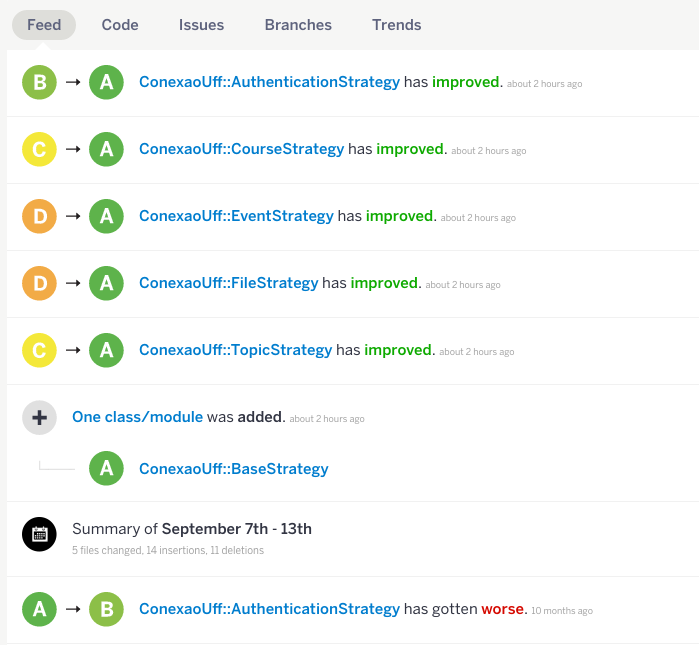
\includegraphics[scale=0.4]{3_7}
    \caption{\textit{Feed} do projeto no \textit{Code Climate} }
    \label{figura7}
\end{figure}

A plataforma ainda conta com uma avaliação geral, chamada de \textit{grade point average} (GPA). Esta avaliação é gerada pela média das notas de todos os arquivos analisados, atribuindo um peso diferente a cada um deles dependendo da quantidade de linhas de código. A GPA varia de zero a quatro, sendo quatro a melhor avaliação possível.

A interface do serviço oferece alguns gráficos interessantes para tornar mais simples o gerenciamento do repositório. Como mostrado na figura \ref{figura8}, contém dados do IntegraUFF, ele informa o GPA ao longo do tempo, o \textit{Breakdown over time}, o qual utiliza um código de cores para identificar as notas individuais de cada arquivo e o \textit{Churn vs Quality}, já explicado anteriormente.  

\begin{figure}[H]
    \centering
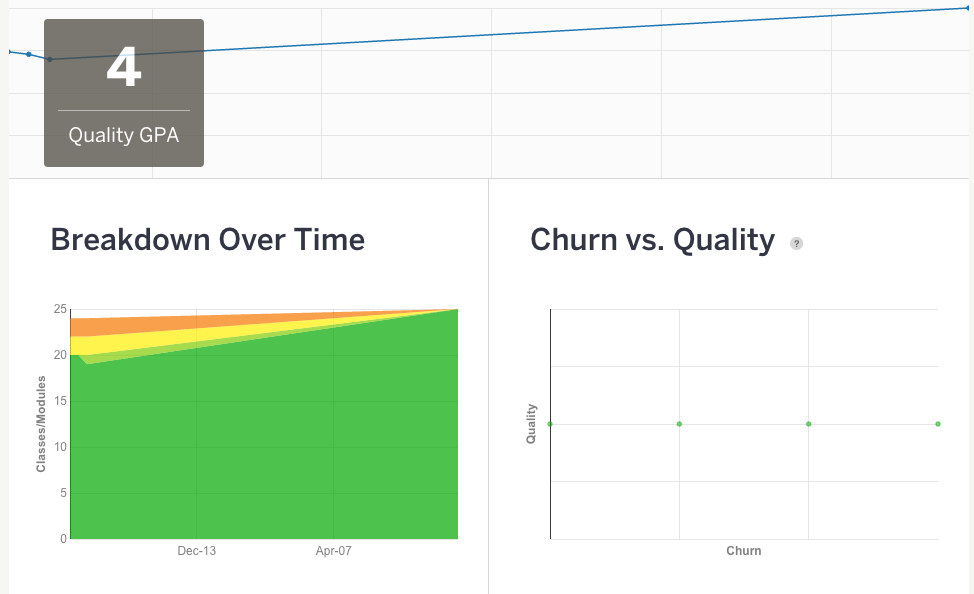
\includegraphics[scale=0.45]{3_8}
    \caption{Gráficos gerados pelo \textit{Code Climate} }
    \label{figura8}
\end{figure}